% Provenance (never printed): see sources/outline_sources.md (Year 2: ore deposits ---
% magmatic, hydrothermal, sedimentary and supergene deposits; grade and tonnage; exploration).
% Deposit descriptions from the USGS Mineral Deposit Models for Resource Assessment
% (Scientific Investigations Report 2010-5070, chapters A, B, C, E, I, L, N, O, Q), USGS
% Open-File Report 03-077 (orogenic gold) and Grabreck et al. 2022 (kimberlites); the grade and
% tonnage data of the world's porphyry copper deposits from USGS Open-File Report 2008-1155
% (dataset bachelor-2-porphyry-cu). Ledger rows in sources/ledger/book4.md; curves and numbers
% from figdata/bachelor-2/ores.py and the Book 4 second-writer scratch calculator calc/ch29.py.
% Geology and sourced numbers only: no advocacy.
\chapter{Gisements de minerai}\label{ch:b2:ore-deposits}

Le cuivre représente environ \qty{0.006}{\percent} de la croûte~; on l'extrait de roches qui en
contiennent environ \qty{0.5}{\percent}. Toute mine de cuivre exploite donc une roche environ
quatre-vingts fois plus riche que la croûte qui l'entoure, et chaque \omterm{def:b2:ore-deposits:deposit}{gisement} est
l'œuvre d'un concentrateur naturel~: un \omterm{def:b2:magma-emplacement:magma}{magma} qui a séparé un liquide sulfuré, une saumure chaude
qui a dissous des métaux et les a déposés dans une fracture, une rivière qui a trié les grains
lourds des grains légers, une pluie qui a lessivé le sommet d'un corps minéralisé et redéposé son
cuivre plus bas. Ce chapitre suit ces concentrateurs, mesure ensuite leurs produits --- quelle quantité de minerai, à quelle \omterm{def:b2:ore-deposits:grade}{teneur} --- et se termine par la façon dont on découvre les \omterm{def:b2:ore-deposits:deposit}{gisements}.
% ledger: perkins:ore-grades

\begin{recall}
\textbf{Des volumes scolaires}~: \omterm{def:b2:ore-deposits:deposit}{gisement} et \omterm{def:b2:ore-deposits:cf}{facteur de concentration}, filon, \omterm{def:b2:ore-deposits:placer}{placer}, réserve et
ressource~; circulation hydrothermale et fumeurs noirs aux dorsales. \textbf{Des livres de chimie}~:
minerai~; solubilité, ions complexes et oxydoréduction. \textbf{Du volume de première année}~: la
vitesse de chute d'un grain et la loi de Stokes~; latérite~; évaporite. \textbf{Du
\cref{ch:b2:elements-in-the-earth}}~: \omterm{def:b2:elements-in-the-earth:goldschmidt}{élément chalcophile}, \omterm{def:b2:elements-in-the-earth:partition}{coefficient de partage
minéral--liquide}. \textbf{Du \cref{ch:b2:magmatic-differentiation}}~: \omterm{def:b2:magmatic-differentiation:cumulate}{intrusion litée} et \omterm{def:b2:magmatic-differentiation:cumulate}{cumulat}.
\textbf{Du \cref{ch:b2:precambrian-earth}}~: \omterm{def:b2:precambrian-earth:bif}{formation de fer rubanée} (BIF), \omterm{def:b2:precambrian-earth:craton}{craton}.
\textbf{Des livres de mathématiques}~: les lois normale et log-normale, et la fonction de
répartition normale $\Phi$.
\end{recall}

\section{Minerai, teneur et concentration}\label{sec:b2:ore-deposits:grade}

\begin{definition}[Gangue]\label{def:b2:ore-deposits:ore}
Dans un minerai, la \emph{gangue}\index{gangue} est tout ce qui n'a aucune valeur économique~: les
minéraux de roche, hydrothermaux et d'altération qui accompagnent les minéraux utiles, séparés
d'eux et rejetés pendant le traitement.
\end{definition}

Dans un \omterm{def:b2:ore-deposits:deposit}{gisement} de cuivre porphyrique, principale source mondiale de cuivre, plus de
\qty{98}{\percent} du minerai est constitué de \omterm{def:b2:ore-deposits:ore}{gangue}, et les minéraux de cuivre forment le reste.
% ledger: usgs10b:share

\begin{definition}[Teneur, teneur de coupure, tonnage]\label{def:b2:ore-deposits:grade}
La \emph{teneur}\index{teneur} d'un volume de roche est la fraction massique de l'élément ou du
minéral utile qu'il contient~: en pour cent pour les métaux de base, en grammes par tonne pour l'or,
l'argent et les éléments du groupe du platine. La \emph{teneur de coupure}\index{teneur de coupure}
est la plus faible teneur à laquelle un bloc de roche est compté comme minerai~; en dessous, le bloc
est stérile. Le \emph{tonnage}\index{tonnage} d'un \omterm{def:b2:ore-deposits:deposit}{gisement} est la masse de roche au-dessus de la
teneur de coupure~; avec sa teneur moyenne $\bar g$, il donne le métal contenu, $M = T\bar g$.
\end{definition}

Le \omterm{def:b2:ore-deposits:grade}{tonnage} et la \omterm{def:b2:ore-deposits:grade}{teneur} d'un \omterm{def:b2:ore-deposits:deposit}{gisement} ne sont donc pas deux faits sur la roche, mais deux réponses
à une même question, posée pour une \omterm{def:b2:ore-deposits:grade}{teneur de coupure} donnée. Batu Hijau, un \omterm{def:b2:ore-deposits:hydrothermal}{gisement de porphyre
cuprifère} et aurifère d'Indonésie, est annoncé à \qty{914}{Mt} à \qty{0.53}{\percent} de cuivre
au-dessus d'une coupure de \qty{0.3}{\percent}, et à \qty{1640}{Mt} à \qty{0.44}{\percent} dans une
compilation mondiale qui retient la coupure la plus basse disponible~: abaisser la coupure presque
double le \omterm{def:b2:ore-deposits:grade}{tonnage} et abaisse la \omterm{def:b2:ore-deposits:grade}{teneur} moyenne. Dans un \omterm{def:b2:ore-deposits:deposit}{gisement} sédimentaire zinc--plomb, le
\omterm{def:b2:ore-deposits:deposit}{gisement} de Tom, au Canada, une baisse de la \omterm{def:b2:ore-deposits:grade}{teneur de coupure} d'environ un pour cent de zinc et de plomb réunis multiplierait les réserves par cinq.
% ledger: usgs10b:cutoffs, usgs08:tonnage-def, usgs10n:sedex

\begin{definition}[Facteur de concentration]\label{def:b2:ore-deposits:cf}
Le \emph{facteur de concentration}\index{facteur de concentration} d'un élément dans un minerai est
le rapport $\mathrm{CF} = g/a$ de sa \omterm{def:b2:ore-deposits:grade}{teneur} $g$ à son abondance $a$ dans un réservoir de référence,
dont il faut indiquer le choix~: la croûte continentale entière, la croûte continentale supérieure, ou la roche à partir de laquelle le \omterm{def:b2:ore-deposits:deposit}{gisement} s'est formé.
\end{definition}

Le facteur dépend de la référence. Pour \qty{0.006}{\percent} de cuivre dans la croûte et
\qty{0.5}{\percent} dans le minerai, on obtient un facteur de 83~; avec la croûte continentale
supérieure, \qty{28}{ppm}, et la \omterm{def:b2:ore-deposits:grade}{teneur} moyenne des porphyres cuprifères de 2008,
\qty{0.44}{\percent}, on obtient 157. L'or, à \qty{1.5}{ng/g} dans la croûte supérieure et exploité
à quelques grammes par tonne, a des facteurs de plusieurs milliers~; le fer, à plusieurs pour cent
dans la croûte et exploité à environ \qty{50}{\percent}, n'a besoin que d'un facteur d'une dizaine.
% ledger: perkins:ore-grades, rg03:ucc-trace, usgs10b:share, earle:ore-grades, earle:iron-grade

\begin{definition}[Gisement]\label{def:b2:ore-deposits:deposit}
Un \emph{gisement}\index{gisement} est un corps de roche dans lequel des processus naturels ont
concentré un élément ou un minéral à une \omterm{def:b2:ore-deposits:grade}{teneur} supérieure à la coupure, sur un \omterm{def:b2:ore-deposits:grade}{tonnage} assez grand
pour être extrait avec profit. Il est à la fois un objet géologique, défini par les processus qui
l'ont formé, et un objet économique, défini par les prix, les coûts et les techniques.
\end{definition}

Parce qu'il a une part économique, la taille d'un \omterm{def:b2:ore-deposits:deposit}{gisement} varie avec le temps. Les ressources
identifiées d'un élément sont les concentrations dont l'extraction est faisable aujourd'hui ou
pourrait le devenir~; ses réserves sont la part qui pouvait être extraite de façon économique au
moment où elles ont été déterminées. Les réserves mondiales de cuivre étaient de \qty{280}{Mt} en
1970~; environ \qty{697}{Mt} ont été extraits depuis, et elles s'élevaient à \qty{980}{Mt} en 2024.
% ledger: usgs:mcs-reserves

\begin{proposition}[Bilan de masse d'un gisement]\label{prop:b2:ore-deposits:mass-balance}
Un \omterm{def:b2:ore-deposits:deposit}{gisement} qui contient une masse $M$ d'un élément à la \omterm{def:b2:ore-deposits:grade}{teneur} moyenne $g$ a été alimenté par une
source dans laquelle l'élément avait une abondance $a$. Si le processus de concentration a extrait
une fraction $\eta \leq 1$ de l'élément de la source et l'a livré au \omterm{def:b2:ore-deposits:deposit}{gisement}, la masse de roche source traitée est
\begin{equation}
m_{\mathrm{source}} = \frac{M}{\eta\,a} = \frac{\mathrm{CF}}{\eta}\, T ,
\label{eq:b2:ore-deposits:mass-balance}
\end{equation}
avec $T = M/g$ le \omterm{def:b2:ore-deposits:grade}{tonnage} et $\mathrm{CF} = g/a$~: au moins CF tonnes de roche source par tonne de minerai.
\end{proposition}

\begin{proof}
La source a perdu $\eta\,a\,m_{\mathrm{source}}$ de l'élément et le \omterm{def:b2:ore-deposits:deposit}{gisement} en a reçu $M$~; en égalant
les deux, on obtient la première forme, et $M = gT$ donne la seconde. Comme $\eta \leq 1$, $m_{\mathrm{source}} \geq
\mathrm{CF}\,T$.
\end{proof}

Bingham Canyon, le \omterm{def:b2:ore-deposits:deposit}{gisement} porphyrique montré ci-dessous, est annoncé à \qty{3230}{Mt} à
\qty{0.882}{\percent} de cuivre, soit \qty{28.5}{Mt} de cuivre. Son facteur par rapport à la croûte
supérieure est 315, et même un procédé parfaitement efficace aurait dû drainer \num{1.02e12} tonnes
de croûte supérieure moyenne, soit environ \qty{377}{km^3}~: un cube de \qty{7.2}{km} de côté.
Les processus de formation des minerais sont donc des processus qui font passer une grande quantité
de matière --- \omterm{def:b2:magma-emplacement:magma}{magma}, eau, sédiment --- par un petit volume où l'élément est piégé.
% ledger: data:b4-porphyry-cu, rg03:ucc-trace
% values: 28.49 Mt; CF 315; 1.0175e12 t; 377 km3 at 2.7 t/m3; side 7.22 km (calc/ch29.py)

\begin{omfigure}
\centering
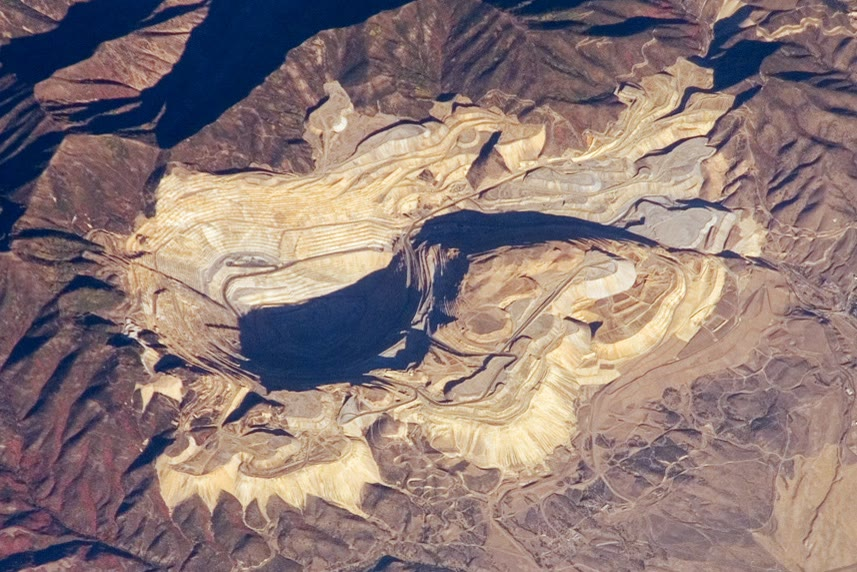
\includegraphics[width=0.5\linewidth]{images/book4/b2-29-bingham-canyon-iss.jpg}
\par\smallskip{\small La fosse de Bingham Canyon, Utah, vue depuis la Station spatiale internationale
(2007)~: plus de \qty{4}{km} de large et \qty{1200}{m} de profondeur, creusée en gradins de 16 à
\qty{25}{m} de hauteur dans un \omterm{def:b2:ore-deposits:deposit}{gisement} porphyrique cuprifère~; les collines à sommets plats qui
l'entourent sont des stériles. Photographie~: NASA, équipage de l'Expédition 15 (domaine public)}.
\end{omfigure}
% ledger: photo:b2-29-bingham

\begin{definition}[Types de gisements]\label{def:b2:ore-deposits:types}
Un \emph{type de gisement}\index{type de gisement} est une classe de \omterm{def:b2:ore-deposits:deposit}{gisements} qui partagent un
cadre géologique, une roche hôte, une forme, une minéralogie de minerai et un processus de
formation, de sorte qu'une description de la classe prédit où ses membres se trouvent. Les types se
répartissent en quatre familles selon le processus~: magmatique (le métal est concentré par un \omterm{def:b2:magma-emplacement:magma}{magma}
pendant qu'il cristallise ou se sépare en deux liquides), hydrothermale (par un fluide aqueux chaud),
sédimentaire (par le transport et le dépôt de sédiments, ou la précipitation depuis l'eau à la
surface), et supergène (par l'altération d'un \omterm{def:b2:ore-deposits:deposit}{gisement} antérieur).
\end{definition}

\section{Gisements magmatiques}\label{sec:b2:ore-deposits:magmatic}

\textbf{Chromite dans les \omterm{def:b2:magmatic-differentiation:cumulate}{intrusions litées}.} La chromite, seule source commerciale de chrome,
se concentre en lits de chromitite massive, contenant plus de \qty{90}{\percent} de chromite, dans
les parties inférieures ultramafiques des \omterm{def:b2:magmatic-differentiation:cumulate}{intrusions litées}. Les intrusions mesurent de 2 à
\qty{180}{km} de large et jusqu'à \qty{15}{km} d'épaisseur, et les lits vont de moins d'un
centimètre à 5--\qty{8}{m}~; ensemble, ils renferment l'essentiel des réserves mondiales de chrome,
et le complexe du Bushveld, rencontré au \cref{ch:b2:magmatic-differentiation}, est aujourd'hui le
seul exploité pour la chromite. Leur origine, une couche de \omterm{def:b2:magmatic-differentiation:cumulate}{cumulat} poussée dans le champ de la
chromite par le \omterm{def:b2:magmatic-differentiation:open}{mélange de magmas} ou par un changement de pression ou d'état d'oxydation, reste débattue.
% ledger: usgs10e:chromite

\textbf{Sulfures de nickel, de cuivre et d'éléments du groupe du platine.} Un \omterm{def:b2:magma-emplacement:magma}{magma} mafique ou ultramafique, produit
par une fusion du manteau à fort degré (\qty{20}{\percent} à \qty{25}{\percent} ou davantage, avec plus de
\qty{12}{\percent} de MgO en masse), monte sous-saturé en soufre. S'il assimile du soufre de la croûte, ou s'il
refroidit assez, il devient saturé et un liquide sulfuré immiscible se sépare en gouttelettes. Les métaux chalcophiles
passent dans ces gouttelettes~: le rapport $D$ de leur concentration dans le liquide sulfuré à celle dans
le \omterm{def:b2:magma-emplacement:magma}{liquide silicaté}, de même nature que le coefficient de partage entre un minéral et un liquide de fusion,
vaut de $10^2$ à $10^3$ pour le cuivre et le nickel, et de $10^3$ à $10^4$ pour les éléments du groupe du platine.
La quantité de métal qu'une gouttelette rassemble dépend alors de la quantité de \omterm{def:b2:magma-emplacement:magma}{magma} qu'elle rencontre.
% ledger: usgs10i:r-factor

\begin{proposition}[Facteur R]\label{prop:b2:ore-deposits:r-factor}
Soit une unité de masse de liquide sulfuré qui se sépare d'une masse $R$ de \omterm{def:b2:magma-emplacement:magma}{magma} silicaté, le
\emph{facteur R}\index{facteur R}, et atteint avec lui l'équilibre, en système fermé~; soit
$C_L$ la concentration d'un métal dans le \omterm{def:b2:magma-emplacement:magma}{magma} avant la séparation du sulfure, et $D$ son coefficient
de partage sulfure--silicate. Alors la concentration du métal dans le sulfure est
\begin{equation}
C_S = C_L\,\frac{D\,(R + 1)}{R + D} .
\label{eq:b2:ore-deposits:r-factor}
\end{equation}
Pour $R \gg D$, $C_S \to D\,C_L$~; pour $R \ll D$, $C_S \approx (R + 1)\,C_L$.
\end{proposition}

\begin{proof}
Le système de masse $R + 1$ contenait $(R + 1)C_L$ de métal avant la séparation. Après celle-ci, le silicate
contient $R\,C_{\mathrm{sil}}$ et le sulfure $C_S$, avec $C_S = D\,C_{\mathrm{sil}}$ à l'équilibre.
La conservation donne $(R + 1)C_L = R\,C_S/D + C_S = C_S\,(R + D)/D$, d'où
\eqref{eq:b2:ore-deposits:r-factor}. Si $R \gg D$, $(R + 1)/(R + D) \to 1$~; si $R \ll D$,
$D/(R + D) \to 1$.
\end{proof}

Les deux limites expliquent l'existence de deux types de minerais sulfurés. Quand $R \ll D$, le sulfure
capte presque tout le métal du \omterm{def:b2:magma-emplacement:magma}{magma} qu'il rencontre, et $C_S$ croît avec $R$~; quand $R \gg D$, il est
saturé à $D\,C_L$ et davantage de \omterm{def:b2:magma-emplacement:magma}{magma} n'ajoute rien. Le nickel et le cuivre, dont $D$ vaut quelques
centaines, atteignent leur plafond pour $R$ de quelques centaines à quelques milliers, soit l'intervalle
de la plupart des minerais nickel--cuivre~; le platine et le palladium, dont $D$ est voisin de $10^4$,
continuent de gagner jusqu'à $R$ de \num{10000} à \num{100000}. Les minerais riches en éléments du
groupe du platine, comme le Merensky Reef du Bushveld et certains minerais de Norilsk, témoignent donc
d'une faible masse de sulfure lessivée par une très grande masse de \omterm{def:b2:magma-emplacement:magma}{magma} (exercices~\ref{exo:b2:ore-deposits:5} et~\ref{exo:b2:ore-deposits:11}).
% ledger: usgs10i:r-factor

\textbf{Kimberlites et diamants.} La plupart des diamants, et presque tous ceux qui sont exploités,
se sont formés à la base de la lithosphère continentale épaisse, dans les racines des \omterm{def:b2:precambrian-earth:craton}{cratons}~; les
\omterm{def:b2:magma-emplacement:magma}{magmas} kimberlitiques, venus de plus de 120 à \qty{150}{km} de profondeur et montant à jusqu'à
\qty{20}{m.s^{-1}}, les amènent à la surface assez vite pour survivre. Les kimberlites font éruption
de préférence à travers une lithosphère épaisse et ancienne, c'est là que s'orientent les prospections de diamants.
% ledger: grabreck22:kimberlite

\textbf{Pegmatites.} Les pegmatites lithium--césium--tantale sont des \omterm{def:b2:magma-emplacement:bodies}{dykes} granitiques enrichis en
ces éléments rares, engendrées dans les \omterm{def:b2:himalaya-andes:types}{orogènes de collision}~; elles cristallisent vers 350 à
\qty{550}{\celsius}, température remarquablement basse pour un liquide granitique, en quelques jours
à quelques années, et forment d'énormes cristaux --- un cristal de spodumène mesurait \qty{14}{m} de long.
Leurs minéraux de lithium, spodumène, pétalite et lépidolite, fournissent environ un quart du lithium mondial.
% ledger: usgs10o:lct

\section{Gisements hydrothermaux}\label{sec:b2:ore-deposits:hydrothermal}

\begin{definition}[Fluide hydrothermal et types de gisements hydrothermaux]\label{def:b2:ore-deposits:hydrothermal}
Un \emph{fluide hydrothermal}\index{fluide hydrothermal} est un fluide aqueux chaud, libéré par un
\omterm{def:b2:magma-emplacement:magma}{magma}, par des \omterm{def:b2:metamorphic-facies:reaction}{réactions métamorphiques}, ou issu d'eau de mer chauffée, d'eau météorique ou de
saumure de bassin, qui dissout, transporte et dépose des éléments en traversant la roche. Les
principaux \omterm{def:b2:ore-deposits:types}{types de gisements} hydrothermaux sont~:
\begin{itemize}
  \item le \emph{gisement de porphyre cuprifère}\index{gisement de porphyre cuprifère}~: un grand corps à faible \omterm{def:b2:ore-deposits:grade}{teneur} de veinules
        et de sulfures de cuivre disséminés dans et autour d'un petit stock porphyrique, formé par des fluides magmatiques
        à moins de quelques kilomètres de la surface au-dessus d'une zone de subduction~;
  \item le \emph{gisement épithermal}\index{gisement épithermal}~: filons et disséminations d'or--argent
        formés à moins d'environ \qty{1.5}{km} de la surface, vers 100 à
        \qty{300}{\celsius}, dans les arcs volcaniques~;
  \item le \emph{amas sulfuré volcanogène}\index{amas sulfuré volcanogène}
        (VMS)~: une lentille de sulfures massifs formée sur ou juste sous le fond marin, à un évent
        hydrothermal dans un cadre volcanique sous-marin~;
  \item le \emph{gisement sédimentaire exhalatif}\index{gisement sédimentaire exhalatif} (SEDEX)~:
        sulfures de zinc et de plomb lités dans des schistes marins d'un \omterm{def:b2:basins-compared:types}{bassin de rift}, précipités sur ou
        juste sous le fond marin à partir de saumures de bassin remontant le long de failles~;
  \item le \emph{gisement de type Mississippi Valley}\index{gisement de type Mississippi Valley} (MVT)~:
        sulfures de zinc et de plomb remplaçant des carbonates de plate-forme, épigénétiques et sans lien
        avec l'activité magmatique, déposés par des saumures de bassin~;
  \item le \emph{gisement d'or orogénique}\index{gisement d'or orogénique}~: filons de quartz aurifères dans
        des ceintures métamorphiques, le long de failles majeures, déposés par des fluides de faible
        salinité et riches en CO$_2$, d'origine métamorphique.
\end{itemize}
\end{definition}
% ledger: usgs10b:form, usgs10q:epithermal, usgs10c:vms, usgs10n:sedex, usgs10a:mvt, drew03:orogenic

\textbf{Transport et dépôt.} La plupart des métaux sont transportés dans les fluides hydrothermaux sous forme
de complexes~: le zinc, le plomb et le cuivre en complexes chlorurés, de sorte que la salinité contrôle leur
solubilité, et l'or, dans les fluides réduits, en complexes soufrés tels que AuHS(H$_2$S)$_3$. Un fluide
lâche sa charge quand sa solubilité baisse~: lorsqu'il se refroidit~; lorsqu'il bout à mesure que sa pression
chute, en perdant H$_2$S et CO$_2$ et en changeant de pH~; lorsqu'il se mêle à un fluide de composition différente
--- une saumure rencontrant une eau riche en H$_2$S précipite de la sphalérite et de la galène presque
aussitôt~; et lorsqu'il réagit avec la roche encaissante, ce qui modifie son pH ou son état d'oxydation.
Chaque \omterm{def:b2:ore-deposits:types}{type de gisement} est une combinaison particulière de fluide, de voie de circulation et de piège.
% ledger: usgs10n:sedex, drew03:orogenic

\textbf{Porphyres cuprifères.} Les \omterm{def:b2:ore-deposits:deposit}{gisements} de porphyre fournissent environ \qty{60}{\percent} du cuivre mondial
et renferment environ \qty{65}{\percent} de ses ressources. Ils sont centrés sur de petits stocks cylindriques
ou des essaims de \omterm{def:b2:magma-emplacement:bodies}{dykes}, sommets de \omterm{def:b2:magma-emplacement:bodies}{plutons} plus grands, mis en place à moins de 5--\qty{10}{km} de profondeur
dans des arcs au-dessus de zones de subduction, le cadre du \cref{ch:b2:magmatic-series}. Un \omterm{def:b2:ore-deposits:deposit}{gisement} mesure
de \num{0.1} à \qty{1}{km} de large, pour une hauteur comparable~; la roche altérée peut s'étendre sur \qty{10}{km}
ou plus autour de lui. Au fur et à mesure que le \omterm{def:b2:magma-emplacement:magma}{magma} cristallise, un fluide contenant \qty{3}{\percent}
à \qty{5}{\percent} de sel en masse s'en sépare~; en remontant et en se décomprimant, il se scinde en une saumure
et une vapeur, qui portent toutes deux des métaux, et sa surpression fracture la roche. Des veines de quartz
précipitent vers 700 à \qty{500}{\celsius}, et la réaction du fluide avec la roche délimite les zones d'altération,
comme dans la coupe ci-dessous. Comme ils se forment peu profondément dans les marges actives, où l'érosion
est rapide, plus de \qty{90}{\percent} des \omterm{def:b2:ore-deposits:deposit}{gisements} de porphyre connus sont cénozoïques ou mésozoïques.
% ledger: usgs10b:share, usgs10b:form, usgs10b:fluids, usgs10b:alteration

\begin{omfigure}
\centering
\begin{tikzpicture}[x=1.15cm, y=1.15cm, font=\small]
\begin{scope}
\clip (-2.9,-3.6) rectangle (2.9,0);
% propylitic halo
\fill[omLithBasalt!45] (0,-1.25) ellipse (2.45 and 1.55);
% sodic-calcic deep flanks
\fill[omExo!25] (-1.75,-2.55) ellipse (0.45 and 0.38);
\fill[omExo!25] (1.75,-2.55) ellipse (0.45 and 0.38);
% sericitic shell
\fill[yellow!35] (0,-1.05) ellipse (1.15 and 1.15);
% potassic core
\fill[omProp!40] (0,-1.45) ellipse (0.68 and 0.85);
% ore shell
\draw[omThm, line width=1.1pt, densely dashed] (0,-1.3) ellipse (0.92 and 0.98);
% advanced argillic lithocap
\fill[omDef!30] (-1.05,0) .. controls (-0.6,-0.5) and (0.6,-0.5) .. (1.05,0) -- cycle;
\draw[omDef!70] (-1.05,0) .. controls (-0.6,-0.5) and (0.6,-0.5) .. (1.05,0);
\end{scope}
% pluton and stock
\fill[omLithGranite] (-2.6,-3.6) .. controls (-2.2,-2.9) and (-0.9,-2.6) .. (-0.3,-2.6)
  -- (-0.3,-1.25) arc[start angle=180, end angle=0, radius=0.3] -- (0.3,-2.6)
  .. controls (0.9,-2.6) and (2.2,-2.9) .. (2.6,-3.6) -- cycle;
\draw[black!60] (-2.6,-3.6) .. controls (-2.2,-2.9) and (-0.9,-2.6) .. (-0.3,-2.6)
  -- (-0.3,-1.25) arc[start angle=180, end angle=0, radius=0.3] -- (0.3,-2.6)
  .. controls (0.9,-2.6) and (2.2,-2.9) .. (2.6,-3.6);
% epithermal veins
\foreach \x in {1.45,1.65,1.85} \draw[omDef, line width=1pt] (\x,-0.02) -- (\x+0.12,-0.7);
% palaeosurface
\draw[black, line width=0.8pt] (-2.9,0) -- (2.9,0);
\node[anchor=south west, font=\scriptsize] at (-2.9,0) {paléosurface};
% labels
\draw[black!50] (0.6,-0.15) -- (1.2,0.25) -- (3.0,0.25) node[anchor=west, text=black] {argillique avancée};
\draw[black!50] (1.95,-0.3) -- (3.0,-0.3) node[anchor=west, text=black] {veines épithermales};
\draw[black!50] (1.05,-0.8) -- (3.0,-0.8) node[anchor=west, text=black] {séricitique};
\draw[black!50] (0.85,-1.25) -- (3.0,-1.25) node[anchor=west, text=omThm] {coquille de minerai de cuivre};
\draw[black!50] (0.45,-1.7) -- (3.0,-1.7) node[anchor=west, text=black] {potassique};
\draw[black!50] (1.05,-2.15) -- (3.0,-2.15) node[anchor=west, text=black] {propylitique};
\draw[black!50] (2.1,-2.6) -- (3.0,-2.6) node[anchor=west, text=black] {sodico--calcique};
\draw[black!50] (1.5,-3.15) -- (3.0,-3.15) node[anchor=west, text=black] {pluton et stock porphyrique};
\end{tikzpicture}
\par\smallskip{\small Système porphyrique cuprifère en coupe (dessin, non à l'échelle)~: la zone potassique au cœur,
profonde et chaude~; la zone séricitique vers le haut et vers l'extérieur, où la pyrite est abondante~; la coquille
de minerai de cuivre entre elles~; le halo propylitique à faible ou moyenne profondeur, autour~; l'altération
sodico--calcique sur les flancs profonds~; un chapeau argileux avancé et, dans certains systèmes, des veines
épithermales près de la surface.}
\end{omfigure}
% ledger: usgs10b:alteration

\textbf{Or épithermal.} Au-dessus de certains systèmes porphyriques, et dans les arcs volcaniques
en général, les mêmes fluides atteignent les \qty{1.5}{km} supérieurs de la croûte
vers 100 à \qty{300}{\celsius}, où ils bouillent et se mêlent aux eaux souterraines~; ils
déposent or et argent dans des veines de quartz, avec une altération qui témoigne de fluides
presque neutres (adulaire, illite) ou très acides (kaolinite, dickite, pyrophyllite).
% ledger: usgs10q:epithermal, usgs10q:alteration

\textbf{Sulfures massifs sur le fond marin.} L'eau de mer entraînée dans la croûte chaude d'une dorsale ou
d'un arc ressort aux évents sous forme de fumeurs noirs vers \qty{350}{\celsius}, observés pour la première
fois sur la dorsale du Pacifique Est en 1979. Là où le champ d'évents dure, ses sulfures édifient un monticule~;
le minerai contient plus de \qty{40}{\percent} de sulfures, au-dessus d'un stockwerk de veines qui
marque le conduit d'alimentation. Les métaux sont zonés selon la température~: fer et cuivre à la base chaude,
zinc, fer, plomb et baryum au sommet et aux marges plus froids, comme dans le monticule dessiné à la
section suivante. Les \omterm{def:b2:ore-deposits:hydrothermal}{amas sulfurés volcanogènes} vont de petites poches de moins d'une tonne aux \qty{1.5}{Gt}
de Rio Tinto en Espagne, et, par l'âge, de \qty{3.55}{\Ga} aux \omterm{def:b2:ore-deposits:deposit}{gisements} qui se forment aujourd'hui.
% ledger: usgs10c:vms

\textbf{Saumures de bassin~: SEDEX et MVT.} Les saumures de bassin, à \qty{10}{\percent} à \qty{30}{\percent} de
sels dissous, chauffées à 100--\qty{200}{\celsius} par l'enfouissement, transportent zinc et plomb sous forme de
complexes chlorurés et forment les deux types logés dans des sédiments. Les \omterm{def:b2:ore-deposits:deposit}{gisements} SEDEX se forment là où la
saumure émerge dans un bassin restreint et réducteur, le long d'une faille de rift, et rencontre le sulfure d'hydrogène,
en produisant des boues sulfurées laminées~; ils renferment plus de la moitié des réserves mondiales de zinc
et de plomb. Les \omterm{def:b2:ore-deposits:deposit}{gisements} MVT se forment là où la saumure, chassée hors d'un bassin, atteint une plate-forme
carbonatée à sa marge et la remplace entre 75 et environ \qty{200}{\celsius}~; ils contiennent \qty{38}{\percent}
du plomb et du zinc des \omterm{def:b2:ore-deposits:deposit}{gisements} logés dans des sédiments, avec environ dix fois plus de zinc que de plomb.
% ledger: usgs10n:sedex, usgs10a:mvt

\textbf{Or orogénique.} Dans les ceintures métamorphiques, les \omterm{def:b2:metamorphic-facies:reaction}{réactions de dévolatilisation} libèrent
un fluide presque neutre, de faible salinité et riche en CO$_2$~; canalisé le long de failles majeures,
il dépose des veines de quartz aurifères vers \qty{350}{\celsius} et entre 4 et \qty{12}{km}
de profondeur. Les veines se prolongent sur de grandes hauteurs~: \qty{3.2}{km} à Kolar, en Inde.
% ledger: drew03:orogenic

\section{Gisements sédimentaires et supergènes}\label{sec:b2:ore-deposits:sedimentary}

\begin{definition}[Placer]\label{def:b2:ore-deposits:placer}
Un \emph{placer}\index{placer} est un \omterm{def:b2:ore-deposits:deposit}{gisement} sédimentaire de minéraux denses et résistants,
concentrés par une eau ou un vent en mouvement, car, à taille égale, ils se déposent
plus vite et sont entraînés moins facilement que les grains de quartz qui les entourent.
\end{definition}

Les minéraux plus denses que 2.85 environ sont dits lourds, contre 2.65 pour le quartz~: ilménite et zircon vers 4.7,
magnétite 5.2, or de 15 à 19.3. Selon la loi de Stokes, la vitesse de chute d'un grain croît avec son excédent de masse
volumique $\rho_s - \rho_w$, onze fois plus grand pour l'or que pour le quartz~; l'or d'une taille donnée se comporte
donc comme du quartz trois fois plus gros (exercice~\ref{exo:b2:ore-deposits:3})~; l'or reste en général dans les
graviers de rivière reposant sur le substratum, tandis que l'ilménite, le rutile et le zircon atteignent les plages
et les dunes. Les \omterm{def:b2:ore-deposits:grade}{teneurs} des sables à minéraux lourds sont exprimées en pourcentage massique de minéraux lourds.
% ledger: usgs10l:heavy, usgs:gold-placer

Les sédiments chimiques sont aussi des minerais. Les \omterm{def:b2:precambrian-earth:bif}{formations de fer rubanées} (BIF) du \cref{ch:b2:precambrian-earth},
précipitées à mesure que le fer dissous des océans s'oxydait, sont un minerai courant de fer~; les évaporites
fournissent la halite et les sels de potassium~; les latérites, résidus d'une altération tropicale profonde,
concentrent l'aluminium sous forme de bauxite. L'altération améliore aussi des \omterm{def:b2:ore-deposits:deposit}{gisements} plus anciens.
% ledger: earle:bif, usgs:bauxite

\begin{definition}[Enrichissement supergène, chapeau de fer]\label{def:b2:ore-deposits:supergene}
\emph{Enrichissement supergène}\index{enrichissement supergène} est la concentration d'un métal par
des eaux souterraines descendantes~: au-dessus de la nappe, des eaux oxygénées et acides dissolvent
le métal des sulfures d'un corps minéralisé, et en dessous, en conditions réductrices, le déposent
de nouveau, surtout en remplaçant les sulfures primaires. Un \emph{chapeau de fer}\index{chapeau de fer}
est la roche poreuse riche en oxydes de fer laissée en surface au-dessus d'un corps sulfuré
altéré, dont les sulfures sont remplacés par de la goethite, de l'hématite et de la jarosite.
\end{definition}

Dans les \omterm{def:b2:ore-deposits:deposit}{gisements} de porphyre, le chapeau lessivé au-dessus de la nappe atteint parfois plusieurs centaines de mètres
d'épaisseur~; en dessous, des zones de sulfures enrichis en chalcocite, épaisses de quelques dizaines à plusieurs
centaines de mètres, atteignent plus de \qty{1.5}{Gt} à 0.4 à \qty{1.7}{\percent} de cuivre, toujours plus riches
que le minerai primaire, hypogène, sous-jacent. Les oxydes de fer d'un \omterm{def:b2:ore-deposits:supergene}{chapeau de fer} et d'un chapeau lessivé
conservent les textures des sulfures qu'ils ont remplacés, et guident la prospection en profondeur~; les chapeaux
de fer et leur coloration ferrugineuse ont révélé aux premiers mineurs de nombreux \omterm{def:b2:ore-deposits:deposit}{gisements} de sulfures massifs.
% ledger: usgs10b:supergene, usgs10c:vms

\begin{omfigure}
\centering
\begin{minipage}[b]{0.46\linewidth}\centering
\begin{tikzpicture}[x=1cm, y=1cm, font=\scriptsize]
\fill[omHist!55] (0,4.0) rectangle (1.8,5.2);
\fill[omMeth!30] (0,3.0) rectangle (1.8,4.0);
\fill[black!55] (0,1.8) rectangle (1.8,3.0);
\fill[black!18] (0,0) rectangle (1.8,1.8);
\draw (0,0) rectangle (1.8,5.2);
\draw[omDef, line width=1pt, densely dashed] (-0.25,3.0) -- (2.05,3.0);
\foreach \x in {0.45,0.9,1.35} \draw[omDef, -{Stealth[length=4pt]}] (\x,5.0) -- (\x,3.2);
\node[anchor=west, align=left] at (2.0,4.6) {chapeau de fer et\\chapeau lessivé (oxydes)};
\node[anchor=west, align=left] at (2.0,3.5) {zone d'oxydes\\(malachite)};
\node[anchor=east, text=omDef, align=right] at (-0.25,3.0) {nappe\\phréatique};
\node[anchor=west, align=left] at (2.0,2.4) {zone enrichie\\(chalcocite)};
\node[anchor=west, align=left] at (2.0,0.9) {minerai primaire\\(chalcopyrite\\+ pyrite)};
\node[anchor=south, font=\scriptsize, text=omDef] at (0.9,5.25) {eau acide, Cu$^{2+}$};
\end{tikzpicture}
\end{minipage}\hfill
\begin{minipage}[b]{0.52\linewidth}\centering
\begin{tikzpicture}[x=1cm, y=1cm, font=\scriptsize]
\fill[omSea] (-2.6,1.4) rectangle (2.6,3.2);
\fill[omLithBasalt!60] (-2.6,-1.6) rectangle (2.6,1.4);
% stockwork cone
\fill[omProp!25] (-0.5,-1.6) -- (0.5,-1.6) -- (1.1,0.9) -- (-1.1,0.9) -- cycle;
\foreach \x/\y in {-0.3/-1.2,0.1/-1.0,-0.6/-0.4,0.4/-0.3,-0.1/0.1,0.6/0.4,-0.7/0.5}
  \draw[omProp!80!black] (\x,\y) -- ++(0.35,0.25);
% mound: upper rim and core
\fill[yellow!45] (-1.8,1.4) .. controls (-1.2,2.35) and (1.2,2.35) .. (1.8,1.4) -- cycle;
\fill[omThm!45] (-1.1,1.4) .. controls (-0.7,2.0) and (0.7,2.0) .. (1.1,1.4) -- cycle;
\draw (-1.8,1.4) .. controls (-1.2,2.35) and (1.2,2.35) .. (1.8,1.4);
% chimney and plume
\fill[black!70] (-0.08,2.1) rectangle (0.08,2.55);
\fill[black!45] (0,2.6) circle (0.12) (0.1,2.8) circle (0.16) (0.25,3.0) circle (0.2);
\draw[omDef, -{Stealth[length=4pt]}] (-2.3,2.9) -- (-2.3,0.2) -- (-1.2,-0.9);
\draw[omThm, -{Stealth[length=4pt]}] (0,-1.5) -- (0,1.2);
\node[anchor=west, text=omDef] at (-2.55,3.05) {eau de mer};
\node[anchor=west] at (0.45,2.85) {fumeur noir, \qty{350}{\celsius}};
\draw[black!50] (1.45,1.75) -- (2.0,2.15) node[anchor=west, text=black] {Zn, Fe, Pb, Ba};
\draw[black!50] (0.6,1.6) -- (2.0,1.15) node[anchor=west, text=black] {Fe, Cu};
\node[anchor=west, align=left] at (0.95,-0.4) {stockwerk\\(conduit)};
\node[anchor=north, text=omThm] at (0,-1.6) {fluide chaud};
\end{tikzpicture}
\end{minipage}
\par\smallskip{\small À gauche~: un profil supergène au-dessus d'un corps de sulfures de cuivre (dessin, non à
l'échelle)~: l'eau acide lessive le cuivre au-dessus de la nappe et le redépose sous forme de chalcocite en dessous,
laissant un \omterm{def:b2:ore-deposits:supergene}{chapeau de fer} en surface. À droite~: un monticule de sulfures massifs volcanogènes en coupe
(dessin)~: l'eau de mer chauffée dans la croûte remonte à travers un stockwerk et ressort en fumeur noir~;
le monticule est zoné, du fer et du cuivre à la base chaude jusqu'au zinc, au fer, au plomb et au baryum
au sommet et aux marges.}
\end{omfigure}
% ledger: usgs10b:supergene, usgs10c:vms

\begin{omfigure}
\centering
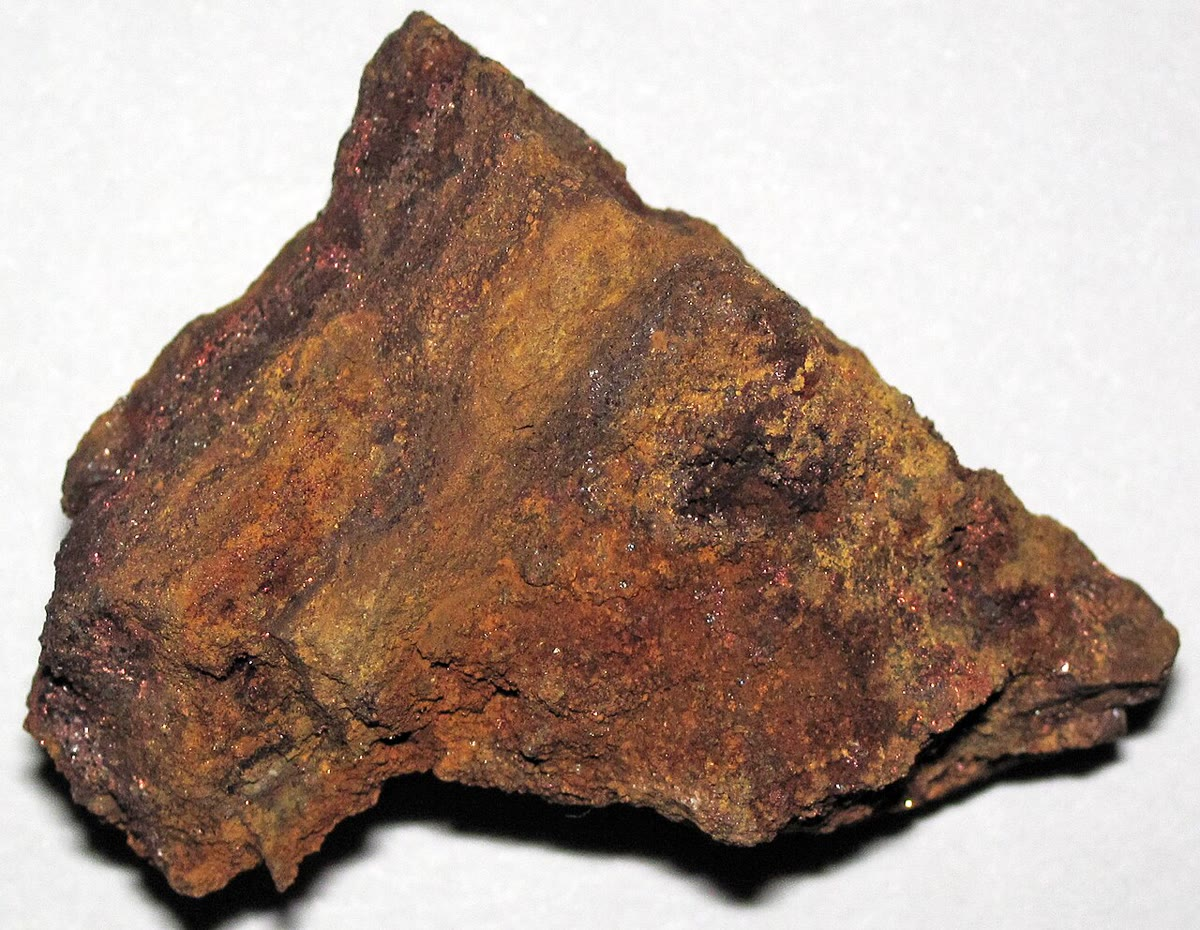
\includegraphics[width=0.4\linewidth]{images/book4/b2-29-flambeau-gossan.jpg}
\par\smallskip{\small \omterm{def:b2:ore-deposits:supergene}{Chapeau de fer} du \omterm{def:b2:ore-deposits:deposit}{gisement} de sulfures massifs de Flambeau, Wisconsin~: une roche poreuse
d'hydroxydes et d'oxydes de fer laissée par l'altération de la pyrite, de la chalcopyrite, de la chalcocite et de la bornite dans un arc volcanique
paléoprotérozoïque~; les petites taches orangées sont du cuivre natif. Photographie~: James St.
John (CC BY 2.0).}
\end{omfigure}
% ledger: photo:b2-29-gossan

\section{Teneur et tonnage}\label{sec:b2:ore-deposits:grade-tonnage}

Une compilation mondiale recense 422 \omterm{def:b2:ore-deposits:hydrothermal}{gisements de porphyre cuprifère} avec leur \omterm{def:b2:ore-deposits:grade}{tonnage}, à la \omterm{def:b2:ore-deposits:grade}{teneur de coupure}
la plus basse disponible, et leur \omterm{def:b2:ore-deposits:grade}{teneur} moyenne en cuivre. Un dixième d'entre eux dépasse \qty{1500}{Mt} et
un dixième contient moins de \qty{33}{Mt}, avec une médiane de \qty{240}{Mt}~; les \omterm{def:b2:ore-deposits:grade}{teneurs} vont de \qty{0.24}{\percent}
à \qty{0.75}{\percent} entre les mêmes déciles, avec une médiane de \qty{0.44}{\percent}. Entre
les déciles, le \omterm{def:b2:ore-deposits:grade}{tonnage} s'étend sur un facteur de 45, la \omterm{def:b2:ore-deposits:grade}{teneur} sur un facteur de 3. Sur des axes logarithmiques,
les deux histogrammes s'approchent de courbes normales, comme le montre la figure ci-dessous~: les logarithmes
du \omterm{def:b2:ore-deposits:grade}{tonnage} ont une moyenne de 2.373 et un écart-type de 0.654, ceux de la \omterm{def:b2:ore-deposits:grade}{teneur} $-0.364$ et 0.199 (logarithmes
en base 10, \omterm{def:b2:ore-deposits:grade}{tonnage} en mégatonnes, \omterm{def:b2:ore-deposits:grade}{teneur} en pour cent). L'ajustement est imparfait~: les \omterm{def:b2:ore-deposits:grade}{teneurs}
sont plus pointues qu'une loi log-normale, et quelques \omterm{def:b2:ore-deposits:deposit}{gisements} très pauvres l'en écartent dans un test formel.
Et les deux grandeurs sont presque indépendantes, avec une corrélation de 0.1 entre leurs logarithmes.
% ledger: usgs08:table1, usgs08:independence, data:b4-porphyry-cu

\begin{omfigure}
\centering
\begin{minipage}[b]{0.49\linewidth}\centering
\begin{tikzpicture}
\begin{axis}[omrecord, width=0.96\linewidth, height=4.5cm, xmin=0.5, xmax=5.0, ymin=0, ymax=80,
  xlabel={tonnage (Mt)}, ylabel={nombre de gisements},
  xtick={1,2,3,4,5}, xticklabels={10,100,1000,$10^4$,$10^5$},
  tick label style={font=\scriptsize}, label style={font=\small}]
% computed in figdata/bachelor-2/ores.py part hist_t; ledger: data:b4-porphyry-cu
\addplot[ybar, bar width=0.22, fill=omDef!35, draw=omDef!70] table[x=log10_t, y=count] {figdata/out/bachelor-2-ores-hist_t.dat};
\addplot[omThm, line width=1pt, smooth] table[x=log10_t, y=fit] {figdata/out/bachelor-2-ores-hist_t.dat};
\end{axis}
\end{tikzpicture}
\end{minipage}\hfill
\begin{minipage}[b]{0.49\linewidth}\centering
\begin{tikzpicture}
\begin{axis}[omrecord, width=0.96\linewidth, height=4.5cm, xmin=-1.2, xmax=0.6, ymin=0, ymax=120,
  xlabel={teneur en cuivre (\%)}, ylabel={nombre de gisements},
  xtick={-1,-0.69897,-0.30103,0,0.30103}, xticklabels={0.1,0.2,0.5,1,2},
  tick label style={font=\scriptsize}, label style={font=\small}]
% computed in figdata/bachelor-2/ores.py part hist_g; ledger: data:b4-porphyry-cu
\addplot[ybar, bar width=0.088, fill=omDef!35, draw=omDef!70] table[x=log10_g, y=count] {figdata/out/bachelor-2-ores-hist_g.dat};
\addplot[omThm, line width=1pt, smooth] table[x=log10_g, y=fit] {figdata/out/bachelor-2-ores-hist_g.dat};
\end{axis}
\end{tikzpicture}
\end{minipage}
\par\smallskip{\small \omterm{def:b2:ore-deposits:grade}{Tonnage} (à gauche) et \omterm{def:b2:ore-deposits:grade}{teneur} en cuivre (à droite) des 422 \omterm{def:b2:ore-deposits:hydrothermal}{gisements de porphyre cuprifère}
de la compilation mondiale, sur axes logarithmiques, avec en rouge les courbes normales de même moyenne
et de même écart-type. Données~: Singer, Berger et Moring (2008), USGS.}
\end{omfigure}

\begin{proposition}[Produit de variables log-normales]\label{prop:b2:ore-deposits:product}
Si $\log_{10} T$ et $\log_{10} g$ sont conjointement normales, de moyennes $\mu_T$ et $\mu_g$,
d'écarts types $\sigma_T$ et $\sigma_g$ et de corrélation $\rho$, alors le métal
contenu $M = Tg/100$ ($g$ en pour cent) est log-normal~: $\log_{10} M$ est normal, avec
\begin{equation}
\mu_M = \mu_T + \mu_g - 2 , \qquad
\sigma_M^2 = \sigma_T^2 + \sigma_g^2 + 2\rho\,\sigma_T\sigma_g .
\label{eq:b2:ore-deposits:product}
\end{equation}
\end{proposition}

\begin{proof}
$\log_{10} M = \log_{10} T + \log_{10} g - 2$. Une combinaison linéaire de variables conjointement
normales est normale (admis dans les volumes de mathématiques)~; sa moyenne est la somme des
moyennes, et sa variance $\operatorname{var}(X + Y) = \operatorname{var} X + \operatorname{var} Y + 2\operatorname{cov}(X, Y)$,
avec $\operatorname{cov}(X, Y) = \rho\,\sigma_T\sigma_g$.
\end{proof}

Pour les \omterm{def:b2:ore-deposits:deposit}{gisements} de porphyre, $\sigma_M = \sqrt{0.654^2 + 0.199^2 + 2 \times 0.1 \times 0.654 \times
0.199} = 0.702$ et $\mu_M = 0.009$~: le \omterm{def:b2:ore-deposits:deposit}{gisement} médian contient environ \qty{1}{Mt} de cuivre, et le métal contenu
se disperse encore plus que le \omterm{def:b2:ore-deposits:grade}{tonnage}. Une loi log-normale d'un étalement si large concentre l'essentiel du métal
dans quelques \omterm{def:b2:ore-deposits:deposit}{gisements}~: le dixième le plus riche contient environ \qty{63}{\percent} du cuivre selon la loi, et
\qty{64}{\percent} dans les données (exercice~\ref{exo:b2:ore-deposits:12}). La figure ci-dessous représente chaque
\omterm{def:b2:ore-deposits:deposit}{gisement} par son \omterm{def:b2:ore-deposits:grade}{tonnage} et sa \omterm{def:b2:ore-deposits:grade}{teneur}, avec des droites de cuivre contenu égal~; Bingham, à \qty{28.5}{Mt},
se trouve entre les droites de 10 et \qty{100}{Mt}.
% ledger: data:b4-porphyry-cu
% values: sd_log10_m 0.702233, mean 0.00857; median M 1.02 Mt; top 10 % share 0.631 (fit) 0.643 (data)

\begin{definition}[Courbe teneur--tonnage]\label{def:b2:ore-deposits:gt}
La \emph{courbe teneur--tonnage}\index{courbe teneur--tonnage} d'un \omterm{def:b2:ore-deposits:deposit}{gisement}
donne, en fonction de la \omterm{def:b2:ore-deposits:grade}{teneur de coupure} $c$, le \omterm{def:b2:ore-deposits:grade}{tonnage} $T(c)$ des
blocs dont la \omterm{def:b2:ore-deposits:grade}{teneur} dépasse $c$ et leur \omterm{def:b2:ore-deposits:grade}{teneur} moyenne $\bar g(c)$.
\end{definition}

\begin{proposition}[Courbe teneur--tonnage d'un gisement log-normal]\label{prop:b2:ore-deposits:gt}
Si les \omterm{def:b2:ore-deposits:grade}{teneurs} des blocs d'un \omterm{def:b2:ore-deposits:deposit}{gisement} de \omterm{def:b2:ore-deposits:grade}{tonnage} total $T_0$ sont log-normales, $\ln g$ étant normal
de moyenne $\mu$ (la \omterm{def:b2:ore-deposits:grade}{teneur} médiane est $e^{\mu}$) et d'écart-type $s$, alors, avec $z = (\mu -
\ln c)/s$,
\begin{equation}
T(c) = T_0\,\Phi(z), \qquad
\bar g(c) = e^{\mu + s^2/2}\,\frac{\Phi(z + s)}{\Phi(z)} ,
\label{eq:b2:ore-deposits:gt}
\end{equation}
et le métal au-dessus de la coupure vaut $M(c) = T_0\,e^{\mu + s^2/2}\,\Phi(z + s)$, soit une fraction $\Phi(z +
s)$ de l'ensemble.
\end{proposition}

\begin{proof}
Posons $\ln g = \mu + s u$, avec $u$ normale centrée réduite. Un bloc est au-dessus de la coupure lorsque $u > (\ln c -
\mu)/s = -z$, ce qui a pour probabilité $1 - \Phi(-z) = \Phi(z)$~; d'où $T(c)$. Le métal au-dessus de la coupure, par unité de \omterm{def:b2:ore-deposits:grade}{tonnage} total, vaut
$\int_{-z}^{\infty} e^{\mu + s u}\,\varphi(u)\,\mathrm{d}u$, avec $\varphi$ la densité de la loi normale centrée réduite. En complétant le carré,
$e^{su}\varphi(u) =
e^{s^2/2}\varphi(u - s)$, de sorte que l'intégrale vaut $e^{\mu + s^2/2}\,[1 - \Phi(-z - s)] = e^{\mu +
s^2/2}\,\Phi(z + s)$. En divisant par $\Phi(z)$, on obtient la \omterm{def:b2:ore-deposits:grade}{teneur} moyenne.
\end{proof}

Lorsque $c \to 0$, la totalité du \omterm{def:b2:ore-deposits:deposit}{gisement} est conservée, à la \omterm{def:b2:ore-deposits:grade}{teneur} moyenne $e^{\mu + s^2/2}$, qui
est supérieure à la médiane. Relever la coupure retire du \omterm{def:b2:ore-deposits:grade}{tonnage} plus vite que du métal, car les blocs
retirés sont les plus pauvres~: dans le \omterm{def:b2:ore-deposits:deposit}{gisement} illustratif de la figure, passer la coupure de
0.2 à \qty{0.5}{\percent} conserve \qty{41}{\percent} du \omterm{def:b2:ore-deposits:grade}{tonnage} mais \qty{61}{\percent} du cuivre.
% values: demo T 876.0/355.0 Mt, M 4.599/2.826 Mt (figdata ores.py gtcurve)

\begin{omfigure}
\centering
\begin{minipage}[b]{0.49\linewidth}\centering
\begin{tikzpicture}
\begin{axis}[omrecord, width=0.96\linewidth, height=5.0cm, xmode=log, ymode=log,
  xmin=2, xmax=50000, ymin=0.05, ymax=2.8, xlabel={tonnage (Mt)}, ylabel={teneur en cuivre (\%)},
  ytick={0.1,0.2,0.5,1,2}, yticklabels={0.1,0.2,0.5,1,2},
  tick label style={font=\scriptsize}, label style={font=\small}]
% computed in figdata/bachelor-2/ores.py parts scatter and iso; ledger: data:b4-porphyry-cu
\addplot[black!45, line width=0.6pt, unbounded coords=jump] table[x=tonnage_mt, y=g01] {figdata/out/bachelor-2-ores-iso.dat};
\addplot[black!45, line width=0.6pt, unbounded coords=jump] table[x=tonnage_mt, y=g1] {figdata/out/bachelor-2-ores-iso.dat};
\addplot[black!45, line width=0.6pt, unbounded coords=jump] table[x=tonnage_mt, y=g10] {figdata/out/bachelor-2-ores-iso.dat};
\addplot[black!45, line width=0.6pt, unbounded coords=jump] table[x=tonnage_mt, y=g100] {figdata/out/bachelor-2-ores-iso.dat};
\addplot[omDef, only marks, mark=*, mark size=0.8pt, opacity=0.7] table[x=tonnage_mt, y=cu_pct] {figdata/out/bachelor-2-ores-scatter.dat};
\addplot[omThm, only marks, mark=square*, mark size=2pt] coordinates {(3230,0.882)};
\node[font=\tiny, text=black!70, fill=white, inner sep=1pt] at (axis cs:4.55,2.2) {0.1};
\node[font=\tiny, text=black!70, fill=white, inner sep=1pt] at (axis cs:45.5,2.2) {1};
\node[font=\tiny, text=black!70, fill=white, inner sep=1pt] at (axis cs:455,2.2) {10};
\node[font=\tiny, text=black!70, fill=white, inner sep=1pt] at (axis cs:4545,2.2) {100 Mt};
\node[font=\scriptsize, text=omThm, anchor=south, fill=white, inner sep=1pt] at (axis cs:3230,1.0) {Bingham};
\end{axis}
\end{tikzpicture}
\end{minipage}\hfill
\begin{minipage}[b]{0.49\linewidth}\centering
\begin{tikzpicture}
\begin{axis}[omrecord, width=0.80\linewidth, height=5.0cm, xmin=0, xmax=1.2, ymin=0, ymax=1000,
  xlabel={teneur de coupure (\%)}, ylabel={tonnage au-dessus de la coupure (Mt)}, axis y line*=left,
  ylabel style={text=omDef}, tick label style={font=\scriptsize}, label style={font=\small}]
% computed in figdata/bachelor-2/ores.py part gtcurve (illustrative deposit)
\addplot[omDef, line width=1.1pt] table[x=cutoff_pct, y=tonnage_mt] {figdata/out/bachelor-2-ores-gtcurve.dat};
\end{axis}
\begin{axis}[width=0.80\linewidth, height=5.0cm, xmin=0, xmax=1.2, ymin=0, ymax=1.6,
  axis y line*=right, axis x line=none, ylabel={teneur moyenne au-dessus de la coupure (\%)},
  ylabel style={text=omThm}, tick label style={font=\scriptsize}, label style={font=\small}]
\addplot[omThm, line width=1.1pt, densely dashed] table[x=cutoff_pct, y=grade_pct] {figdata/out/bachelor-2-ores-gtcurve.dat};
\end{axis}
\end{tikzpicture}
\end{minipage}
\par\smallskip{\small À gauche~: \omterm{def:b2:ore-deposits:grade}{tonnage} et \omterm{def:b2:ore-deposits:grade}{teneur} en cuivre des 422 \omterm{def:b2:ore-deposits:hydrothermal}{gisements de porphyre cuprifère}, avec des droites
de cuivre contenu égal (de 0.1 à \qty{100}{Mt})~; le carré rouge est Bingham Canyon. Données~: Singer, Berger et
Moring (2008), USGS. À droite~: la \omterm{def:b2:ore-deposits:gt}{courbe teneur--tonnage} d'un \omterm{def:b2:ore-deposits:deposit}{gisement} illustratif de \qty{1000}{Mt}, de \omterm{def:b2:ore-deposits:grade}{teneur} médiane
\qty{0.40}{\percent}, $s = 0.60$~: \omterm{def:b2:ore-deposits:grade}{tonnage} au-dessus de la coupure (bleu) et sa \omterm{def:b2:ore-deposits:grade}{teneur} moyenne (rouge,
en tirets), d'après \eqref{eq:b2:ore-deposits:gt}.}
\end{omfigure}

\section{Prospection}\label{sec:b2:ore-deposits:exploration}

Les \omterm{def:b2:ore-deposits:deposit}{gisements} se trouvent grâce aux traces qu'ils laissent au-delà de leur minerai. La zone d'altération d'un système porphyrique
s'étend sur plusieurs kilomètres~; là où la roche affleure, ses minéraux peuvent être cartographiés depuis des avions et des
satellites grâce à leurs spectres infrarouges~; ses métaux se dispersent dans les sols, les sédiments de cours d'eau, les eaux
et les plantes alentour~; et ses sulfures et ses roches altérées modifient les propriétés physiques que mesure la géophysique.
% ledger: usgs10b:form, usgs10b:exploration, usgs10b:remote

\begin{definition}[Anomalie géochimique]\label{def:b2:ore-deposits:exploration}
Une \emph{anomalie géochimique}\index{anomalie géochimique} est une concentration d'un élément,
ou d'un groupe d'éléments, dans un milieu échantillonné --- roche, sol, sédiment
de cours d'eau, eau, plantes --- qui s'écarte du fond géochimique régional, c'est-à-dire
de la gamme de concentrations rencontrée là où aucune minéralisation n'est présente.
\end{definition}

Comme les \omterm{def:b2:ore-deposits:grade}{teneurs}, les concentrations s'étalent sur plusieurs ordres de grandeur, si bien qu'une anomalie
s'apprécie en général sur les logarithmes~; un seuil simple, utilisé à l'exercice~\ref{exo:b2:ore-deposits:9},
est la moyenne des logarithmes du fond augmentée de deux fois leur écart-type. Un échantillon de sédiment
de cours d'eau mélange les sédiments de tout son bassin versant~; une anomalie s'estompe donc vers
l'aval, à mesure que des sédiments propres s'y ajoutent, et le gradient des concentrations pointe vers l'amont,
en direction de la source. Dans les sols au-dessus de pegmatites enfouies, des anomalies de lithium,
de rubidium, de césium, de tantale et d'étain ont été tracées au-dessus de corps qui n'affleurent pas.
% ledger: usgs10b:exploration, usgs10o:lct

Les méthodes géophysiques sont choisies pour le contraste qu'offre un \omterm{def:b2:ore-deposits:types}{type de gisement}. Les sulfures
disséminés font d'une roche un condensateur~: la polarisation provoquée, qui mesure cette chargeabilité,
a été mise au point pour le porphyre cuprifère et répond surtout à la zone séricitique
riche en pyrite, le cœur potassique étant plus pauvre en sulfures. Les levés magnétiques et gravimétriques
cartographient les \omterm{def:b2:magma-emplacement:bodies}{plutons} auxquels les \omterm{def:b2:ore-deposits:deposit}{gisements} sont liés. Aucune méthode ne voit directement
le minerai, et toute interprétation reste non unique tant qu'un forage ne la teste pas.
% ledger: usgs10b:exploration

\begin{method}[De l'analyse à l'estimation d'une ressource]\label{met:b2:ore-deposits:resource}
Les données sont des forages disposés selon une grille à travers le \omterm{def:b2:ore-deposits:deposit}{gisement}~;
leur carotte est décrite et analysée par intervalles de longueur connue.
\begin{enumerate}
  \item \textbf{Composite.} Moyenner les \omterm{def:b2:ore-deposits:grade}{teneurs} sur des longueurs égales, en pondérant chaque analyse par sa
        longueur, de sorte que chaque composite représente le même volume.
  \item \textbf{Modèle.} Découper le \omterm{def:b2:ore-deposits:deposit}{gisement} en blocs et estimer la \omterm{def:b2:ore-deposits:grade}{teneur} de chacun à partir des composites voisins,
        en les pondérant selon la distance et selon la corrélation spatiale des \omterm{def:b2:ore-deposits:grade}{teneurs} (la méthode géostatistique
        du krigeage, admise).
  \item \textbf{Bilan.} Appliquer une coupure~: \omterm{def:b2:ore-deposits:grade}{tonnage} et \omterm{def:b2:ore-deposits:grade}{teneur} moyenne des blocs au-dessus de celle-ci, avec
        la masse volumique de la roche, à chaque niveau de confiance permis par l'espacement des forages.
\end{enumerate}
\end{method}

\begin{inthefield}[Description d'une carotte de forage]
\centering
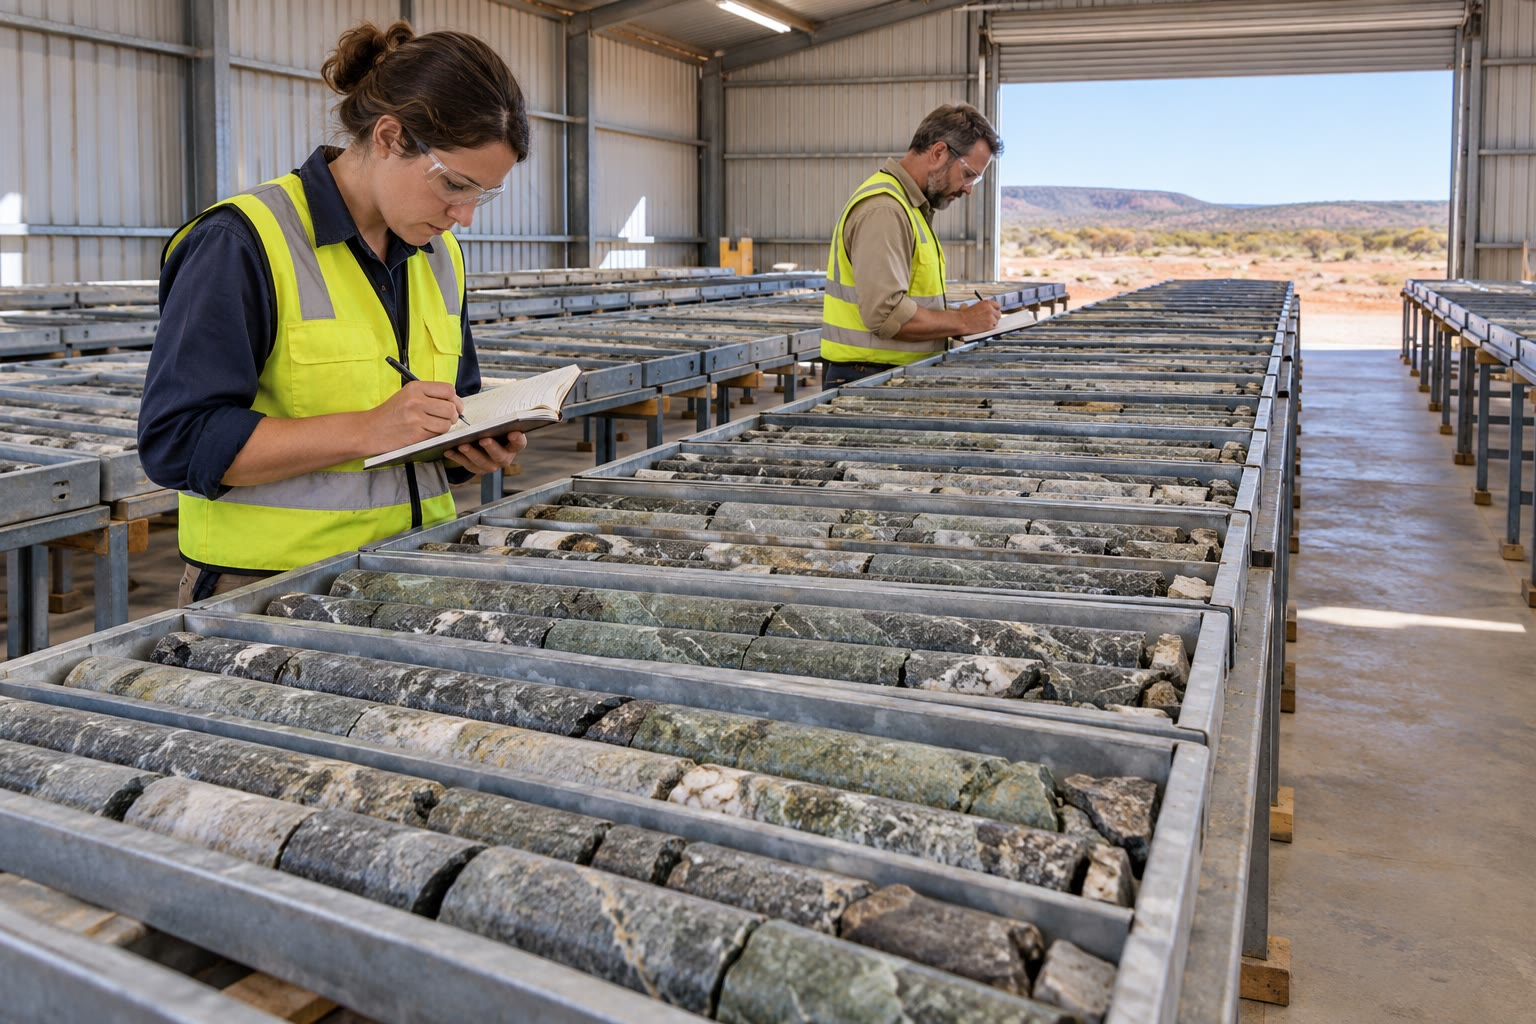
\includegraphics[width=0.56\linewidth]{images/book4/ai/b2-core-shed.jpg}
\par\smallskip{\small Hangar à carottes d'un projet d'exploration. Illustration générée par IA.}
\par\medskip\raggedright
Sur un projet d'exploration, la carotte de chaque forage est disposée dans des plateaux métalliques,
dans l'ordre où elle est sortie du sol. Les géologues parcourent les plateaux, intervalle par intervalle,
et notent la nature de la roche, son altération, les veines qui la recoupent et leur proportion,
ainsi que les sulfures qu'elle contient~; ils marquent l'endroit où la carotte sera sciée et échantillonnée.
La description précède les analyses et leur est comparée~: une zone d'altération ou un type
de veine qui porte le métal devient ce qu'il faut suivre de forage en forage, et, à partir de la description,
les géologues tracent les coupes à partir desquelles les forages suivants sont planifiés.
\end{inthefield}

\section*{Exercices}\label{sec:b2:ore-deposits:exercises}

Données des exercices, sauf mention contraire~: croûte continentale supérieure, cuivre \qty{28}{ppm},
or \qty{1.5}{ng/g}, chrome \qty{92}{ppm}~; la population des \omterm{def:b2:ore-deposits:hydrothermal}{gisements de porphyre
cuprifère} de la \cref{sec:b2:ore-deposits:grade-tonnage}, $\log_{10}$ \omterm{def:b2:ore-deposits:grade}{tonnage} (Mt)
de moyenne 2.373 et d'écart-type 0.654, $\log_{10}$ \omterm{def:b2:ore-deposits:grade}{teneur} (\%) de moyenne $-0.364$ et d'écart-type
0.199, corrélation $\rho = 0.100$. Arrondir à trois chiffres significatifs.
% ledger: rg03:ucc-trace, data:b4-porphyry-cu

\begin{exercise}[$\star$]\label{exo:b2:ore-deposits:1}
Calculer le \omterm{def:b2:ore-deposits:cf}{facteur de concentration} par rapport à la croûte supérieure de~: (a) un minerai de cuivre à
\qty{0.5}{\percent}~; (b) un minerai d'or à \qty{6}{g/t}~; (c) une chromitite de \qty{90}{\percent} de
chromite, en prenant la chromite pour FeCr$_2$O$_4$ (masses atomiques Cr 52.00, Fe 55.85, O 16.00).
\end{exercise}

\begin{exercise}[$\star$]\label{exo:b2:ore-deposits:2}
Batu Hijau est annoncé à \qty{914}{Mt} à \qty{0.53}{\percent} de Cu et \qty{0.40}{g/t} d'Au au-dessus d'une
coupure de \qty{0.3}{\percent}, et à \qty{1640}{Mt} à \qty{0.44}{\percent} de Cu et \qty{0.45}{g/t}
d'Au à la coupure la plus basse disponible. (a) Calculer le cuivre contenu (Mt) et l'or contenu (t) de
chaque estimation. (b) Quels \omterm{def:b2:ore-deposits:grade}{tonnage} et quel cuivre les blocs supplémentaires de la seconde estimation
ajoutent-ils, et à quelle \omterm{def:b2:ore-deposits:grade}{teneur} moyenne~? (c) Pourquoi les deux estimations sont-elles correctes~?
\end{exercise}

\begin{exercise}[$\star$]\label{exo:b2:ore-deposits:3}
Dans la loi de Stokes, la vitesse de chute d'un grain de diamètre $d$ est proportionnelle à $(\rho_s -
\rho_w)\,d^2$. Prendre $\rho_w = 1.00$, quartz 2.65, or 19.3, zircon 4.7 (en
\unit{g.cm^{-3}}). (a) Combien de fois plus vite un grain d'or se dépose-t-il qu'un grain de quartz de même taille~?
(b) Quel est le rapport des diamètres d'un grain d'or et d'un grain de quartz qui se déposent à la même vitesse~?
(c) Quel grain de quartz se dépose comme un grain de zircon de \qty{0.1}{mm}~?
\end{exercise}

\begin{exercise}[$\star$]\label{exo:b2:ore-deposits:4}
Un minerai primaire de cuivre a une \omterm{def:b2:ore-deposits:grade}{teneur} de \qty{0.4}{\percent}. L'altération lessive tout son
cuivre sur une épaisseur de \qty{150}{m} et le redépose dans une couverture d'enrichissement
épaisse de \qty{50}{m} juste en dessous, la masse volumique étant la même. (a) Calculer la \omterm{def:b2:ore-deposits:grade}{teneur}
de la couverture. (b) Même question si seulement \qty{80}{\percent} du cuivre lessivé est redéposé.
(c) Quelle épaisseur lessivée donnerait \qty{1.7}{\percent} avec un redépôt complet~?
\end{exercise}

\begin{exercise}[$\star\star$]\label{exo:b2:ore-deposits:5}
Un \omterm{def:b2:magma-emplacement:magma}{magma} contient \qty{10}{ppb} de platine et \qty{200}{ppm} de nickel~; prendre $D_{\mathrm{Pt}} =
10^4$ et $D_{\mathrm{Ni}} = 500$. (a) À l'aide de \eqref{eq:b2:ore-deposits:r-factor}, calculer les \omterm{def:b2:ore-deposits:grade}{teneurs} en platine (ppm)
et en nickel (\% en masse) du sulfure pour $R = 100$, \num{1000}, \num{10000} et \num{100000}. (b) Trouver leurs limites
pour $R \to \infty$. (c) Expliquer pourquoi un minerai de nickel renseigne peu sur $R$
et un minerai de platine beaucoup.
\end{exercise}

\begin{exercise}[$\star\star$]\label{exo:b2:ore-deposits:6}
À l'aide de \eqref{eq:b2:ore-deposits:product}, pour la population des \omterm{def:b2:ore-deposits:hydrothermal}{gisements de porphyre cuprifère}~: (a) calculer
la moyenne et l'écart-type de $\log_{10} M$, ainsi que le cuivre contenu médian. (b) Quelle fraction des \omterm{def:b2:ore-deposits:deposit}{gisements}
contient plus de \qty{10}{Mt} de cuivre~? Combien sur 422~? (c) Reprendre (b) en négligeant la corrélation.
\end{exercise}

\begin{exercise}[$\star\star$]\label{exo:b2:ore-deposits:7}
Pour le \omterm{def:b2:ore-deposits:deposit}{gisement} illustratif de la figure ($T_0 = \qty{1000}{Mt}$, médiane \qty{0.40}{\percent}, $s = 0.60$),
utiliser \eqref{eq:b2:ore-deposits:gt} pour calculer le \omterm{def:b2:ore-deposits:grade}{tonnage}, la \omterm{def:b2:ore-deposits:grade}{teneur} moyenne et le cuivre contenu
au-dessus des coupures de \qty{0.3}{\percent} et \qty{0.6}{\percent}. Vérifier un point sur la figure.
\end{exercise}

\begin{exercise}[$\star\star$]\label{exo:b2:ore-deposits:8}
Un \omterm{def:b2:ore-deposits:deposit}{gisement} de porphyre contient \qty{5}{Mt} de cuivre. Supposons que son fluide magmatique transporte
\qty{1000}{ppm} de cuivre, dont la moitié se dépose dans le minerai, et que le \omterm{def:b2:magma-emplacement:magma}{magma} libère \qty{3.5}{\percent}
de sa masse sous forme de fluide. (a) Calculer la masse de fluide et celle de \omterm{def:b2:magma-emplacement:magma}{magma} nécessaires.
(b) Calculer le volume du \omterm{def:b2:magma-emplacement:magma}{magma}, de masse volumique \qty{2600}{kg.m^{-3}}. (c) Si le \omterm{def:b2:magma-emplacement:magma}{magma} contenait
\qty{50}{ppm} de cuivre, quelle fraction de ce cuivre s'est-elle retrouvée dans le minerai~?
\end{exercise}

\begin{exercise}[$\star\star$]\label{exo:b2:ore-deposits:9}
Huit sédiments de cours d'eau prélevés sur le fond géochimique donnent un $\log_{10}$ Cu (ppm)
de 1.30, 1.45, 1.38, 1.52, 1.41, 1.35, 1.48 et 1.40. (a) Calculer la moyenne et l'écart-type (population)
des logarithmes, la médiane du fond et le seuil, moyenne plus deux écarts-types, en
ppm. (b) Un affluent drainant \qty{4}{km^2} de terrain minéralisé transporte un sédiment à \qty{400}{ppm}~;
il rejoint un cours d'eau drainant \qty{36}{km^2} à la médiane du fond. En supposant
que chaque kilomètre carré fournit la même masse de sédiment, le sédiment mélangé est-il anomal~?
(c) Jusqu'à quelle surface totale de bassin l'anomalie reste-t-elle au-dessus du seuil~?
\end{exercise}

\begin{exercise}[$\star\star\star$]\label{exo:b2:ore-deposits:10}
(a) Démontrer $e^{su}\varphi(u) = e^{s^2/2}\varphi(u - s)$. (b) En déduire la moyenne d'une variable
log-normale, $e^{\mu + s^2/2}$. (c) Montrer que la fraction du métal au-dessus de la
coupure, $\Phi(z + s)$, dépasse toujours la fraction du \omterm{def:b2:ore-deposits:grade}{tonnage}, $\Phi(z)$, et interpréter.
\end{exercise}

\begin{exercise}[$\star\star\star$]\label{exo:b2:ore-deposits:11}
(a) À partir de \eqref{eq:b2:ore-deposits:r-factor}, calculer le $R$ auquel $C_S$ atteint une fraction $f$
de son plafond $D\,C_L$. (b) Le calculer pour $f = 0.5$ et $0.9$, avec $D = 300$ (nickel) et $D =
10^4$ (platine). (c) Comparer avec les intervalles de $R$ des minerais nickel--cuivre et des récifs riches en éléments
du groupe du platine donnés dans le texte.
\end{exercise}

\begin{exercise}[$\star\star\star$]\label{exo:b2:ore-deposits:12}
(a) Pour une variable log-normale $M$ dont $\ln M$ a un écart-type $s$, montrer que les \omterm{def:b2:ore-deposits:deposit}{gisements} au-dessus
du quantile d'ordre $q$ contiennent une fraction $\Phi\bigl(s - \Phi^{-1}(q)\bigr)$ du métal total. (b) Évaluer
cette fraction pour la population de porphyres et $q = 0.9$. (c) Même question pour $q = 0.99$~; comparer
avec les quatre plus grands \omterm{def:b2:ore-deposits:deposit}{gisements}, qui contiennent \qty{26.6}{\percent} du cuivre de la compilation.
\end{exercise}
% ledger: data:b4-porphyry-cu

\begin{problem}[{Problème du week-end --- Un indice porphyrique}]\label{pb:b2:ore-deposits:1}
Un indice porphyrique (fictif) a été foré. Son forage de découverte a recoupé huit intervalles, du
haut vers le bas (longueur en mètres, \omterm{def:b2:ore-deposits:grade}{teneur} en cuivre en pour cent)~: 30 m à 0.12~; 40 à 0.35~;
50 à 0.62~; 60 à 0.48~; 40 à 0.27~; 30 à 0.81~; 50 à 0.41~; 30 à 0.18. Une étude géostatistique
de tous les forages trouve que les \omterm{def:b2:ore-deposits:grade}{teneurs} des blocs sont log-normales, de médiane \qty{0.38}{\percent}
et $s = 0.55$ pour $\ln g$. Le corps minéralisé est proche d'un cylindre vertical de rayon
\qty{450}{m} et de hauteur \qty{700}{m}, de masse volumique \qty{2.7}{t.m^{-3}}. Utiliser les
données des exercices, et arrondir à trois chiffres significatifs (les probabilités à quatre).

\noindent\textbf{Partie I --- Le forage de découverte.}
\begin{enumerate}
  \item Calculer la longueur du forage échantillonné et sa \omterm{def:b2:ore-deposits:grade}{teneur} moyenne pondérée par la longueur.
  \item Calculer la moyenne arithmétique des huit \omterm{def:b2:ore-deposits:grade}{teneurs}. Pourquoi la moyenne pondérée est-elle la bonne~?
  \item Quelle fraction de la longueur se trouve au-dessus de \qty{0.3}{\percent}, et à quelle \omterm{def:b2:ore-deposits:grade}{teneur} moyenne~?
  \item Calculer le \omterm{def:b2:ore-deposits:cf}{facteur de concentration} de la \omterm{def:b2:ore-deposits:grade}{teneur} moyenne pondérée par rapport à la croûte supérieure.
  \item Faire de même pour l'intervalle le plus riche.
  \item Calculer la \omterm{def:b2:ore-deposits:grade}{teneur} moyenne de tous les blocs du \omterm{def:b2:ore-deposits:deposit}{gisement}. Le forage de découverte est-il représentatif~?
\end{enumerate}

\noindent\textbf{Partie II --- Tonnage au-dessus de la coupure.}
\begin{enumerate}[resume]
  \item Calculer le volume et le \omterm{def:b2:ore-deposits:grade}{tonnage} $T_0$ du corps~; retenir $T_0 = \qty{1200}{Mt}$.
  \item Pour une coupure de \qty{0.3}{\percent}, calculer $z$ et la fraction des blocs au-dessus.
  \item Calculer le \omterm{def:b2:ore-deposits:grade}{tonnage} au-dessus des coupures de 0.2, 0.3 et \qty{0.5}{\percent}.
  \item Calculer la \omterm{def:b2:ore-deposits:grade}{teneur} moyenne au-dessus de la coupure de \qty{0.3}{\percent}.
  \item Faire de même au-dessus de 0.2 et de \qty{0.5}{\percent}.
  \item Lorsqu'on relève la coupure de 0.3 à \qty{0.5}{\percent}, de quels facteurs changent le \omterm{def:b2:ore-deposits:grade}{tonnage} et la
        \omterm{def:b2:ore-deposits:grade}{teneur} moyenne~?
  \item À quelle coupure conserve-t-on la moitié du \omterm{def:b2:ore-deposits:grade}{tonnage}, et quelle est sa \omterm{def:b2:ore-deposits:grade}{teneur} moyenne~?
\end{enumerate}

\noindent\textbf{Partie III --- L'indice parmi les porphyres du monde.}
\begin{enumerate}[resume]
  \item Calculer le cuivre contenu dans tout le corps, à sa \omterm{def:b2:ore-deposits:grade}{teneur} moyenne.
  \item Calculer le score réduit de son \omterm{def:b2:ore-deposits:grade}{tonnage} dans la population mondiale, et son centile.
  \item Faire de même pour sa \omterm{def:b2:ore-deposits:grade}{teneur} moyenne.
  \item Calculer l'écart-type de $\log_{10} M$ avec la corrélation, puis sans elle.
  \item Calculer le centile de son cuivre contenu.
  \item Combien des 422 \omterm{def:b2:ore-deposits:deposit}{gisements} seraient censés contenir davantage de cuivre~?
\end{enumerate}

\noindent\textbf{Partie IV --- Cuivre au-dessus de la coupure.}
\begin{enumerate}[resume]
  \item Calculer le cuivre contenu au-dessus de la coupure de \qty{0.2}{\percent}.
  \item Faire de même au-dessus de \qty{0.5}{\percent}.
  \item Quelle fraction du cuivre se trouve au-dessus de \qty{0.3}{\percent}, et quelle fraction du
        \omterm{def:b2:ore-deposits:grade}{tonnage}~?
  \item Expliquer pourquoi abaisser la coupure en dessous de \qty{0.3}{\percent} ajoute beaucoup de roche et peu
        de cuivre, en utilisant les réponses aux questions 9 et 20.
  \item En résumé, combien de cuivre l'indice contient-il au-dessus de la coupure de \qty{0.3}{\percent}~?
\end{enumerate}
\end{problem}
